\documentclass[aspectratio=169]{beamer}
\usepackage[utf8]{inputenc}
\usepackage{xeCJK}
\usepackage{graphicx}
\usepackage {mathtools}
\usepackage{utopia} %font utopia imported
\usetheme{CambridgeUS}
\usecolortheme{dolphin}

% Russian language
%\usepackage[russian]{babel}
\usepackage[utf8]{inputenc}
\usepackage[T2A, T1]{fontenc}
\usepackage{fontspec}
\usefonttheme{serif}
\setmainfont{Times New Roman}

% set colors
\definecolor{myNewColorA}{RGB}{126,12,110}
\definecolor{myNewColorB}{RGB}{165,85,154}
\definecolor{myNewColorC}{RGB}{203,158,197}
\setbeamercolor*{palette primary}{bg=myNewColorC}
\setbeamercolor*{palette secondary}{bg=myNewColorB, fg = white}
\setbeamercolor*{palette tertiary}{bg=myNewColorA, fg = white}
\setbeamercolor*{titlelike}{fg=myNewColorA}
\setbeamercolor*{title}{bg=myNewColorA, fg = white}
\setbeamercolor*{item}{fg=myNewColorA}
\setbeamercolor*{caption name}{fg=myNewColorA}
\usefonttheme{professionalfonts}
\usepackage{natbib}
\usepackage{hyperref}
%------------------------------------------------------------
%\titlegraphic{\includegraphics[height=1.5cm]{nku-logo.eps}}

\setbeamerfont{title}{size=\large}
\setbeamerfont{subtitle}{size=\small}
\setbeamerfont{author}{size=\small}
\setbeamerfont{date}{size=\small}
\setbeamerfont{institute}{size=\small}
\title[On the problem of repeated supervised learning]{On the problem of repeated supervised learning}
\subtitle{My first scientific paper}
\author[Andrey Veprikov]{Andrey Veprikov \and Anton Khritankov
\and Alexander Afanasyev}

\institute[veprikov.as@phystech.edu]{
MIPT\\
Dolgoprudny, Russia}

\date[Spring 2023]
{Spring 2023}

%------------------------------------------------------------
%This block of commands puts the table of contents at the 
%beginning of each section and highlights the current section:
%\AtBeginSection[]
%{
%  \begin{frame}
%    \frametitle{Contents}
%    \tableofcontents[currentsection]
%  \end{frame}
%}
%\AtBeginSection[]{
%  \begin{frame}
%  \vfill
%  \centering
%  \begin{beamercolorbox}[sep=8pt,center,shadow=true,rounded=true]{title}
%    \usebeamerfont{title}\insertsectionhead\par%
%  \end{beamercolorbox}
%  \vfill
%  \end{frame}
%}
%------------------------------------------------------------

\begin{document}

%The next statement creates the title page.
\frame{\titlepage}
%\begin{frame}
%\frametitle{Содержание}
%\tableofcontents
%\end{frame}
%------------------------------------------------------------
\section{Goals and contributions of paper}
    \begin{frame}{Introduction and Related work}
        \small

        In this research paper, we delve into the intricacies of continuous learning artificial intelligence systems as they interact with and influence their environment. Many authors have dealt with the problem from a narrative perspective \cite{bottou2013counterfactual, sculley2015hidden}, i.e. so far only the problem of multiple learning has been articulated, but nowhere in the literature is a robust analysis of the process presented.

        Repeated supervised learning appears in many machine learning applications, for example in 
        
        \begin{enumerate}
            \item recommendation systems \cite{khritankov2021existence}
    
            \item healthcare \cite{adam2020hidden}
    
            \item predictive policing \cite{ensign2018runaway}
        \end{enumerate}
        
        Contributions of this paper are as follows
        
        \begin{enumerate}
            \item Develop a mathematical model to examine the process of repeated supervised learning, prediction, and dataset updating in presented cases.
        
            \item Conduct several synthetic experiments based on our findings, hoping to contribute to a better understanding of the behavior of continuous learning AI systems.
        \end{enumerate}
        
    \end{frame}

    \begin{frame}{Problem statement}
        \footnotesize
        The object of our research will be the set $\mathbf{R}$ of distribution density functions
    
        \begin{equation*}
            \mathbf{R} := \left\{f : \mathbb{R}^n \rightarrow \mathbb{R}_+ ~\text{and}~ \int\limits_{\mathbb{R}^n}f(x)dx = 1\right\}
        \end{equation*}
    
        and mappings $\text{D}_t \in \mathbb{D}$ as feedback loop mapping. We consider discrete dynamical system \cite{katok1995introduction}:

        \begin{equation}
            \label{system}
            f_{t+1}(x) = \text{D}_t(f_t)(x), \quad \text{for}~ \forall x \in \mathbb{R}^n, t \in \mathbb{N}~\text{ and }~ \text{D}_t \in \mathbb{D}
        \end{equation}

        If $\{\text{D}_t\}_{t=0}^{\infty}$ are independent of time, then \eqref{system} takes the form

        \begin{equation}
            \label{system_new}
            f_{t+1}(x) = \text{D}(f_t)(x), \quad \text{for}~ \forall x \in \mathbb{R}^n, t \in \mathbb{N}
        \end{equation}

        According to Conjecture 1 from \cite{khritankov2021hidden} the positive feedback loop in a system \eqref{system} exists if 

        \begin{equation*}
            \forall f, g \in \mathbf{R} \hookrightarrow \rho(R_H(\text{D}(f)), R_H(\text{D}(g))) \leq \lambda \cdot \rho(R_H(f), R_H(g)),
        \end{equation*}

        where $R_H$ is quality measure of model $H$, $\rho(\cdot, \cdot)$ is a distance metric and $\lambda \in (0; 1)$.       
    \end{frame}

    \begin{frame}{Problem statement}
        \begin{figure}[h!]
            \centering
            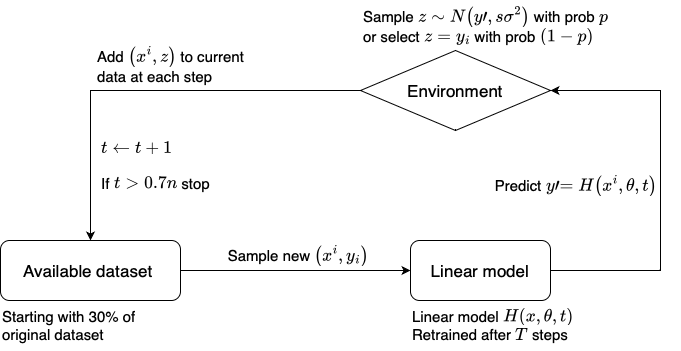
\includegraphics[width=0.49\linewidth]{pictures/Hidden_loop.png}
            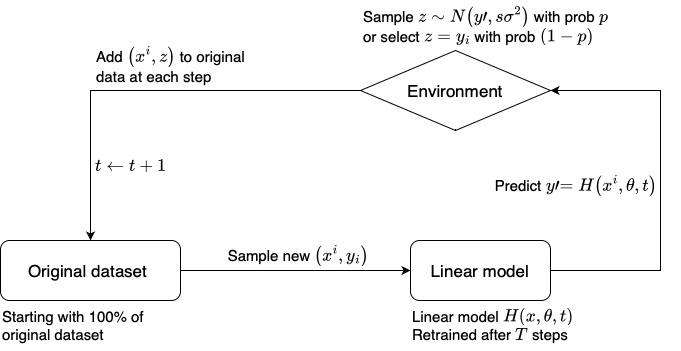
\includegraphics[width=0.49\linewidth]{pictures/Hidden_sample.png}\\
            
            \caption{Simulations of a real systems from \cite{khritankov2021hidden}.}
            \label{w}
        \end{figure}
        
    \end{frame}

\section{Main results}
    \begin{frame}{Assumptions for $\text{D}: \mathbf{R} \to \mathbf{R}$}

        \large{\textcolor{myNewColorA}{\textbf{Theorem 1} (Fact)}}
        \normalsize

        If $f: \mathbb{R}^n \to \mathbb{R}$ such that $f(x) \geq 0$ for almost every $x \in \mathbb{R}^n$ and $\|f\|_1 = \int\limits_{\mathbb{R}^n} f(x) dx = 1$, then there exists a random vector $\mathbf{\xi}$, for which $f$ will be a density distribution function.
        
        \large{\textcolor{myNewColorA}{\textbf{Theorem 2} (Assumptions for $\text{D}: \mathbf{R} \to \mathbf{R}$)}}
        \normalsize
    
        If $\|\text{D}\|_1 = 1, \forall f \in \mathbf{R} \hookrightarrow \text{D}(f)(x) \geq 0$ for almost every $x \in \mathbb{R}^n$, and exists $\text{D}^{-1}$ such that $\|\text{D}^{-1}\|_1 \leq 1$, then $\text{D} : \mathbf{R} \to \mathbf{R}$.\\
    \end{frame}

    \begin{frame}{Limit in a weak sense to $\delta$ or zero function}
        \normalsize{\textcolor{myNewColorA}{\textbf{Theorem 3}}}
        \small

        If $f_t : \mathbb{R} \to \mathbb{R}$ such that $\forall t \in \mathbb{N} \hookrightarrow  \|f_t\|_1 = 1$, $f_t(x) \geq 0$ in almost every point $x \in \mathbb{R}$ and
        \begin{equation*}
            \exists \psi : \mathbb{N} \to \mathbb{R} : \psi(t) \underset{t \to +\infty}{\longrightarrow} +\infty ~\text{ and }~
            \exists g \in L_1(\mathbb{R}) ~\text{ such that }~
        \end{equation*}
        \begin{equation}
            \label{g_and_psi}
            \forall t \in \mathbb{N} ~\forall y \in \mathbb{R} \hookrightarrow f_t\left(\dfrac{y}{\psi(t)}\right) \leq \psi(t) \cdot |g(y)|
        \end{equation}

        Then $f_t(x) \underset{t \to \infty}{\longrightarrow} \delta(x)$ in a weak sense, i.e.

        \begin{equation*}
            \underset{t \to +\infty}{\lim}\left( \text{ } \int\limits_{-\infty}^{+\infty} f_t(x) \phi(x) dx \text{ } \right) = \phi(0),
        \end{equation*}

        where $\phi$ is continuous function with compact support

        If $\psi(t) \underset{t \to +\infty}{\longrightarrow} 0$, then $f_t(x) \underset{t \to \infty}{\longrightarrow} 0$.

        We consider the one-dimensional case because we can compare each operator $\text{D}$ to an operator $\widetilde{\text{D}}$, where $\widetilde{\text{D}}$ transforms density distribution functions of random variables $\|\mathbf{y} - \mathbf{y_{\text{pred}}}\|$
        
    \end{frame}

    \begin{frame}{Important example of $\psi$ and $g$}
        \small
        Important example of operators $\text{D}_t$ for which the following is fulfilled $\text{D}_t(f_0)(x) \underset{t \to \infty}{\longrightarrow} \delta(x)$ is as follows 

        \begin{equation*}
            \text{D}_t(f_0)(x) = t \cdot f_0(t \cdot x)
        \end{equation*}

        Here we take $g(x) = f_0(x)$ and $\psi(t) = t$. 

        \begin{figure}[h!]
            \centering
            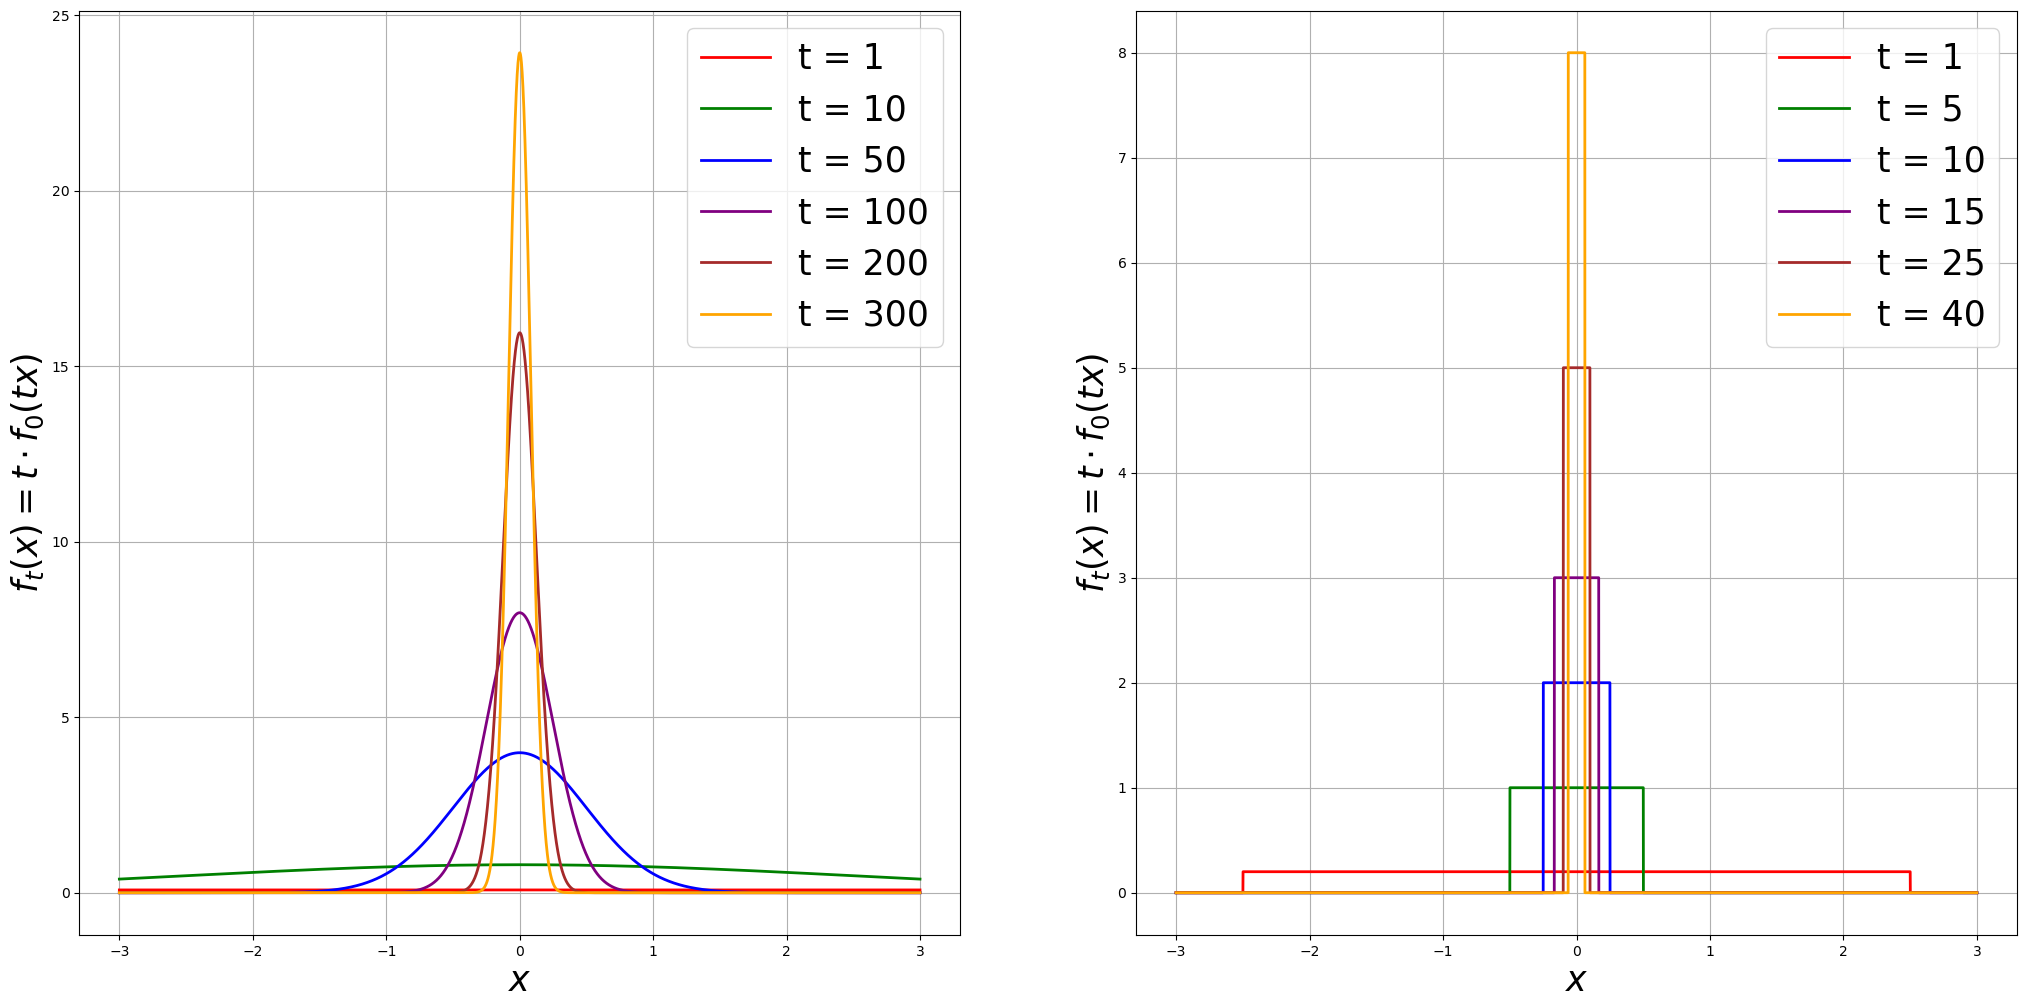
\includegraphics[width=0.55\linewidth]{pictures/example1.png}
            
            Illustration of weak limit to $\delta$ function. $\mathcal{N}(0, 5)$ left, $\mathcal{U}[-2.5, 2.5]$ right.
            \label{example1_fig}
        \end{figure}
        
    \end{frame}

    \begin{frame}{Consequences of the Theorem 3}
        \small
        \textcolor{myNewColorA}{\textbf{Corollary 1} (Experimental $\psi$ determination)}

        If 
            $\forall x \neq 0 \hookrightarrow f_t(x) \underset{t \to \infty}{\longrightarrow} 0$ and $f_t(0) \underset{t \to \infty}{\longrightarrow} +\infty$,
        then we can take
            $\psi(t) = \dfrac{f_t(0)}{|g(0)|}$

        In the following we assume that the operators $\text{D}_t \in \mathbb{D}$ have the form  

        \begin{equation} \label{cool_D}
            \text{D}_t(f_0)(x) = \psi(t) \cdot f_0(\psi(t) \cdot x) ~\text{ and }~ \psi(t) \to +\infty
        \end{equation}
        
        \textcolor{myNewColorA}{\textbf{Corollary 2} (Autonomy criterion)}

        If a system satisfies \eqref{cool_D}, it is autonomous if and only if

        \begin{equation} \label{cong_semigroup}
            \psi(\tau + \kappa) = \psi(\tau) \cdot \psi(\kappa) ~\forall \tau, \kappa \in \mathbb{N}
        \end{equation}

        \textcolor{myNewColorA}{\textbf{Corollary 3} (Decreasing moments)}

        If $\text{D}_t$ have the form \eqref{cool_D}, then all $k$-th moments of random variable $\|\mathbf{y} - \mathbf{y_{\text{pred}}}\|$ (if they exist) are decreasing with speed $\psi(t)^{-k}$, i.e. $\nu_k^t = \psi(t)^{-k} \nu_k^0$, where $\nu_k^t$ is a $k$-th moment on a step $t$.

        If $~\exists q \in [1; +\infty]$ such $\{\nu_k^0\}_{k=1}^{+\infty} \in l_q$, then $\{\nu_k^t\}_{k=1}^{+\infty} \in l_1$ and $\{\nu_k^t\}_{k=1}^{+\infty} \underset{t \to \infty}{\overset{l_1}{\longrightarrow}} 0$

    \end{frame}

    \begin{frame}{Inequality on $\|\text{D}\|_q$}
        \large{\textcolor{myNewColorA}{\textbf{Theorem 4}}}
        \normalsize
        
        Consider 
        \begin{equation*}
            f_A(x) = \dfrac{1}{\lambda(A)} \cdot \textbf{1}_{A}(x),
        \end{equation*}

        where $A \subset \mathbb{R}^n$ is arbitrary set of a non-path measure, $\lambda(A)$ -- the measure of a set $A$.

        Then for all $A \subset \mathbb{R}^n :  0 < \lambda(A) < +\infty$ and for all $1 \leq q \leq +\infty$ such that $\text{D}^t(f_A) \in L_q(\mathbb{R}^n)$ is fulfilled that  

        \begin{equation*}
            \|\text{D}_t\|_q \geq \int\limits_{A} \text{D}_t(f_A)(x)dx
        \end{equation*}

        This theorem gives a sufficient condition that the operators $\text{D}_t$ wouldn't be a contraction mapping in $\|\cdot\|_q$.
    \end{frame}

\section{Experiments}

    \begin{frame}{Experiment setup}
        \begin{figure}[h!]
            \centering
            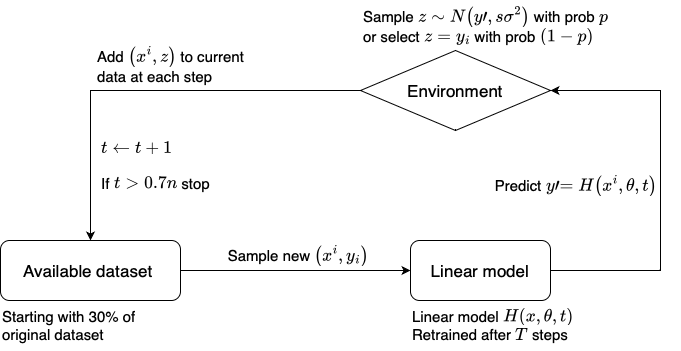
\includegraphics[width=0.49\linewidth]{pictures/Hidden_loop.png}
            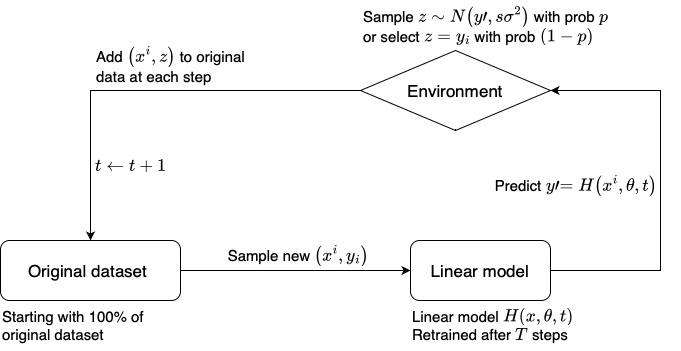
\includegraphics[width=0.49\linewidth]{pictures/Hidden_sample.png}\\
            
            \caption{Sliding window setup (left) and sampling setup (right).}
            \label{w_1}
        \end{figure}
        
    \end{frame}

    \begin{frame}{Analysis of deviation}
        
        \footnotesize
        Every $N$ steps we measured the standard deviation in the $\mathbf{y} - \mathbf{y_{\text{pred}}}$ array, where $\mathbf{y_{\text{pred}}}$ is the predictions of our model on the active dataset. We measured the standard deviation at different \textit{usage} -- the probability with which we take $(\mathbf{x^i}, z_i)$ into the active dataset, and \textit{adherence} -- the parameter by which we multiply $\sigma^2$ when sampling $z_i$. 
        
        \begin{figure}[h!]
            \centering
            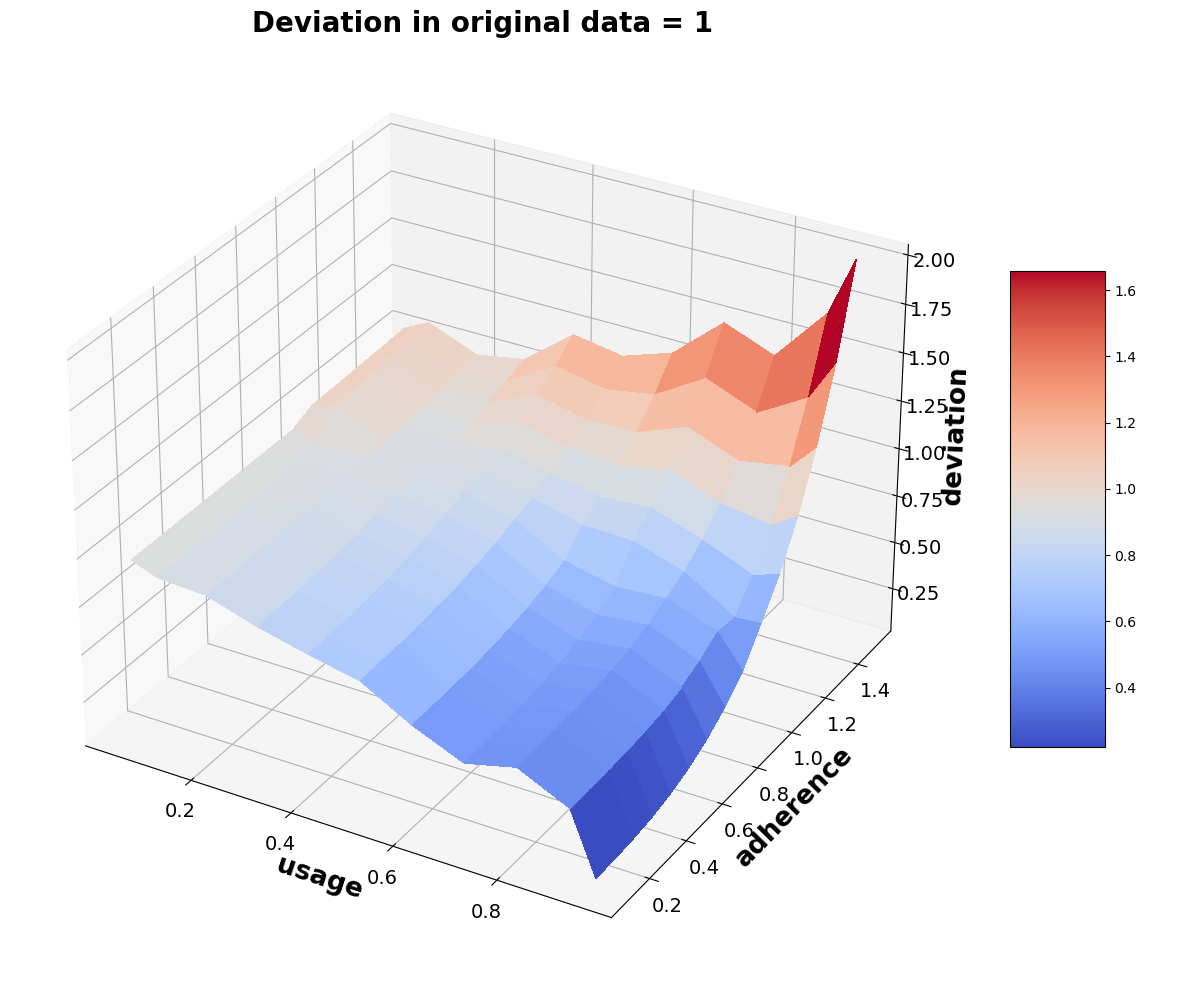
\includegraphics[width=0.3\linewidth]{pictures/3D_plot_loop_1.png}
            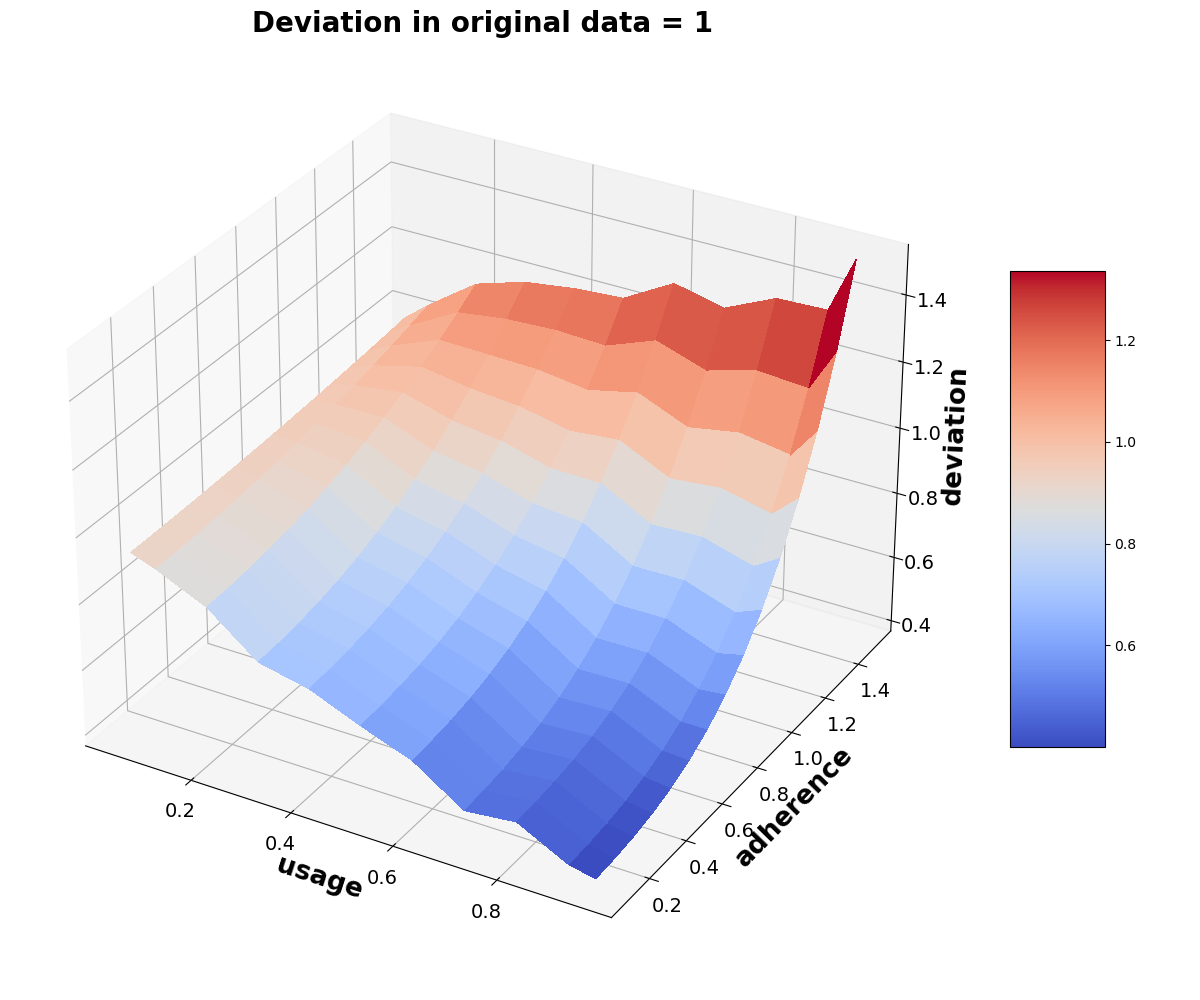
\includegraphics[width=0.3\linewidth]{pictures/3D_plot_sample_1.png}
            
            \caption{Analysis of deviation. Sliding window (left), sampling update (right).}
            \label{3D}
        \end{figure}

        As you can see, as a increases \textit{usage} and decreases \textit{adherence} deviation falls, this is because we start adding less noisy data to the active dataset.
        
    \end{frame}

    \begin{frame}{Exploring the form of the data distribution over time}
        
        \small
        We check our data for belonging to a normal distribution by counting $p$-value from normal test. 
        
        \begin{figure}[h!]
            \centering
            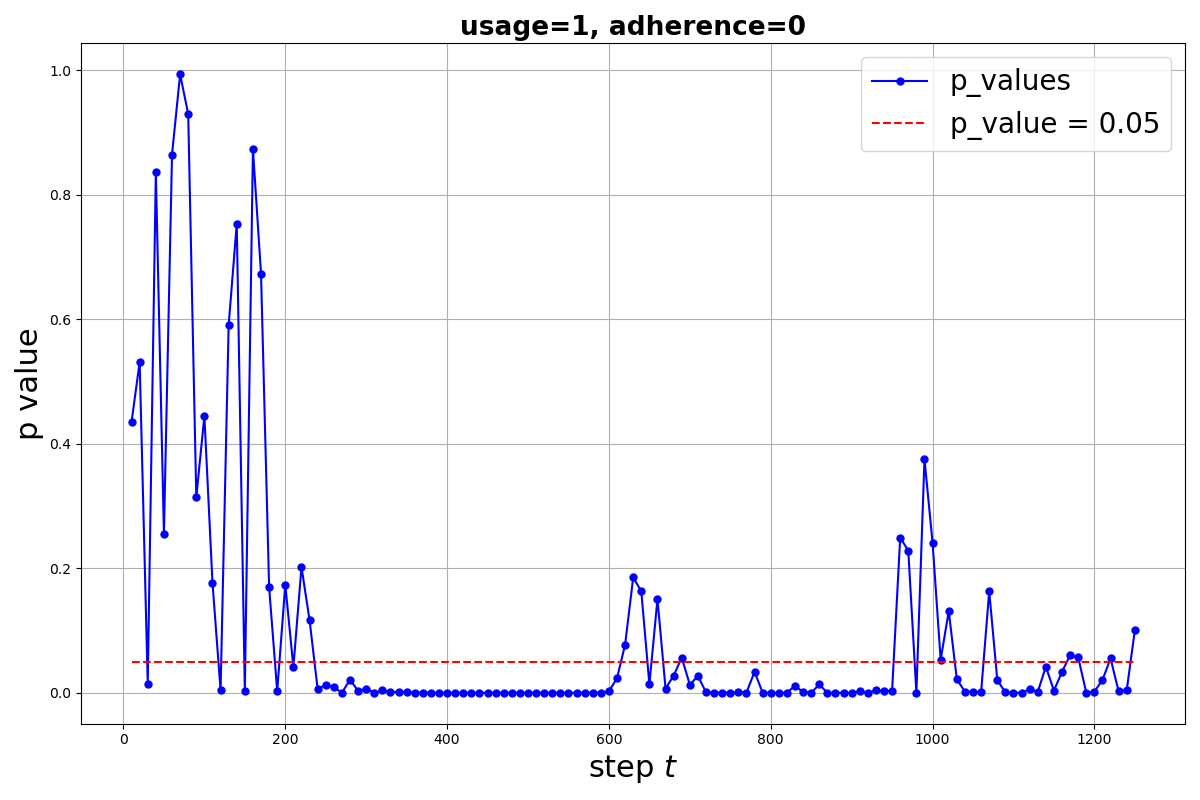
\includegraphics[width=0.45\linewidth]{pictures/p_loop_1_0.png}
            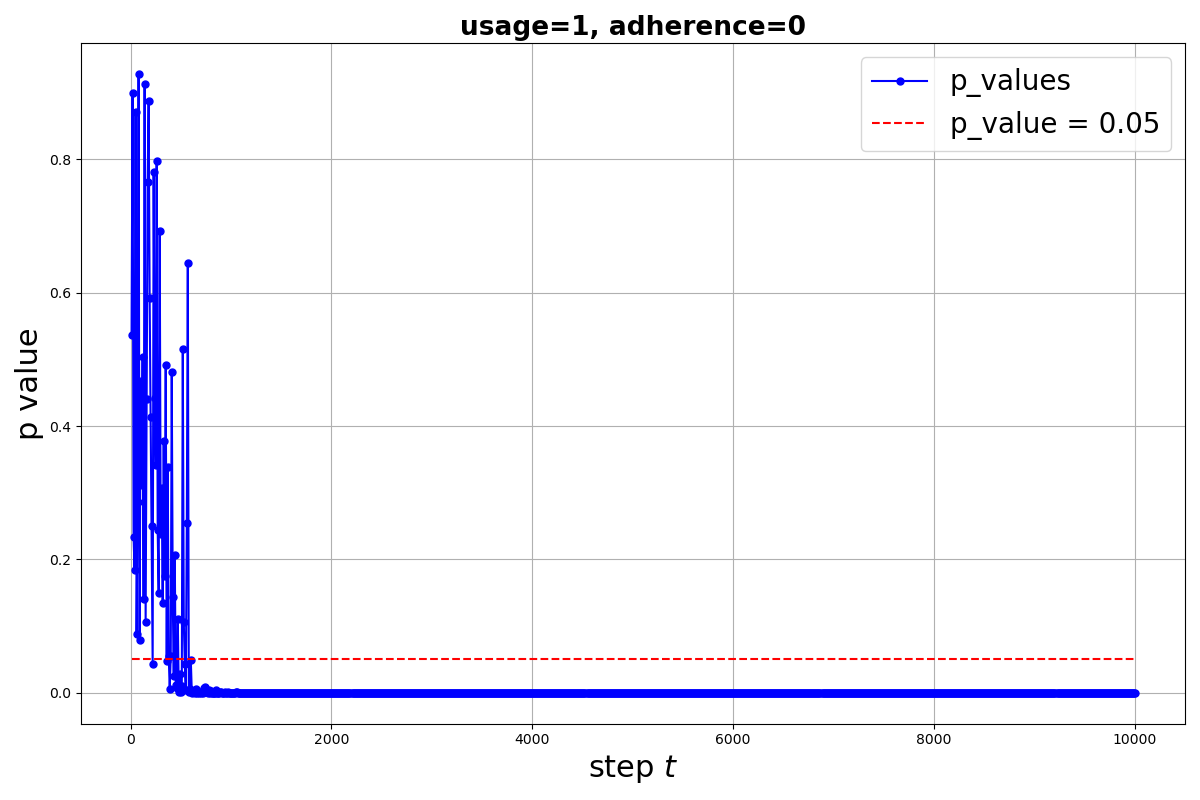
\includegraphics[width=0.45\linewidth]{pictures/p_sample_1_0.png}
            
            \caption{Analysis of $p$-value. Sliding window (left), sampling update (right).}
            \label{p_value}
        \end{figure}

        As you can see, the normality of the data breaks down as $t$ increases.
    \end{frame}
    
    \begin{frame}{Histograms}
        \small
        As you can see, $\mathbf{y} - \mathbf{y_{\text{pred}}}$ is not normally distributed for all experiment types. 
        
        \begin{figure}[h!]
            \centering
            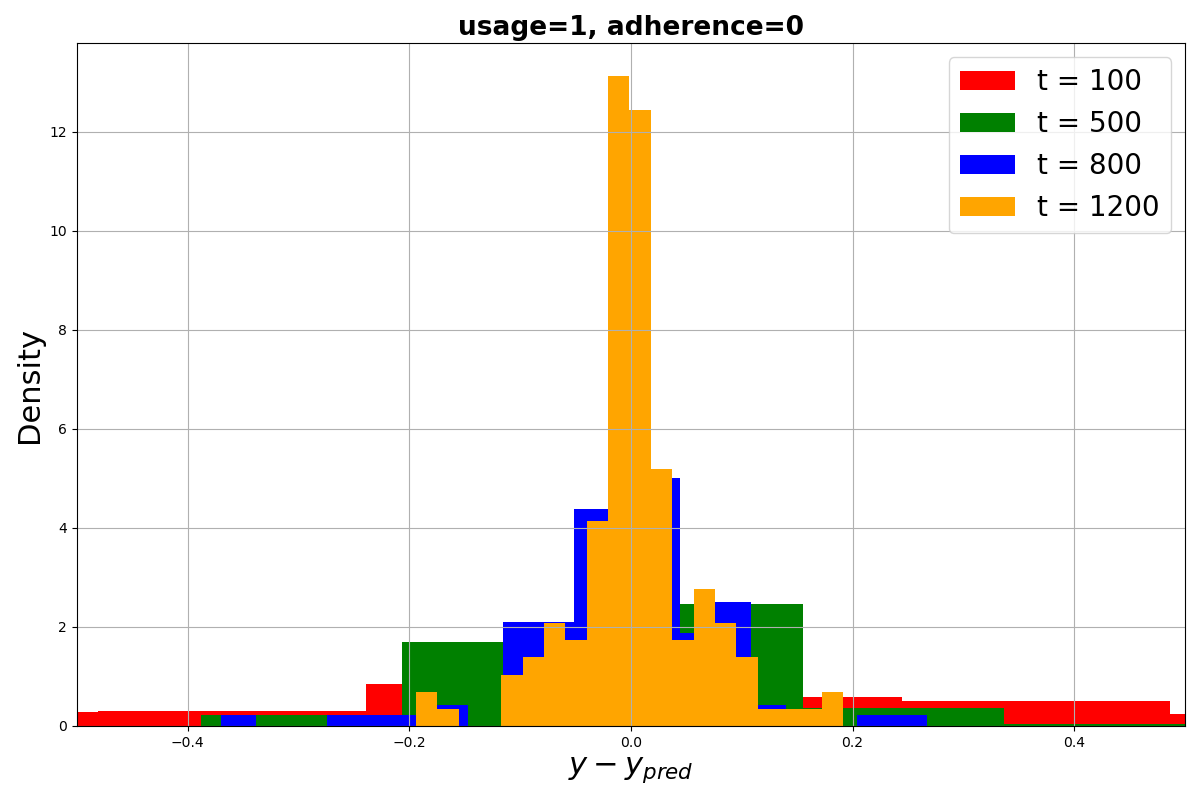
\includegraphics[width=0.45\linewidth]{pictures/hist_loop_1_0.png}
            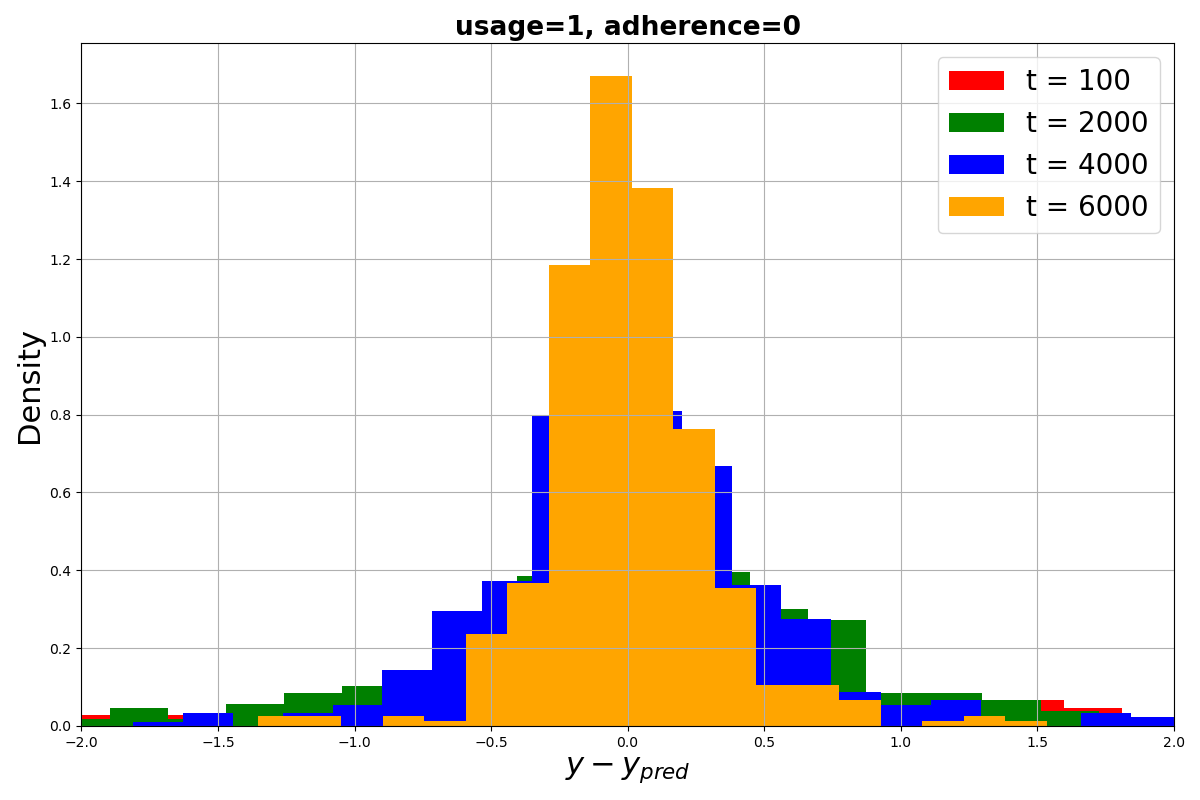
\includegraphics[width=0.45\linewidth]{pictures/hist_sample_1_0.png}
            
            \caption{Histograms for some $t$. Sliding window (left), sampling update (right).}
            \label{hist}
        \end{figure}

        As you can see $\mathbf{y} - \mathbf{y_{\text{pred}}}$ seems to be a mixture of the two distributions
    \end{frame}

    \begin{frame}{Limit to delta function}
        \small
        In this experiment we test the conditions from Theorem 3, i.e. we measure $f_t(0)$ and $\int\limits_{-\kappa}^{\kappa}f_t(x)dx$, where $\kappa$ is sufficiently small. 

        \begin{figure}[h!]
            \centering
            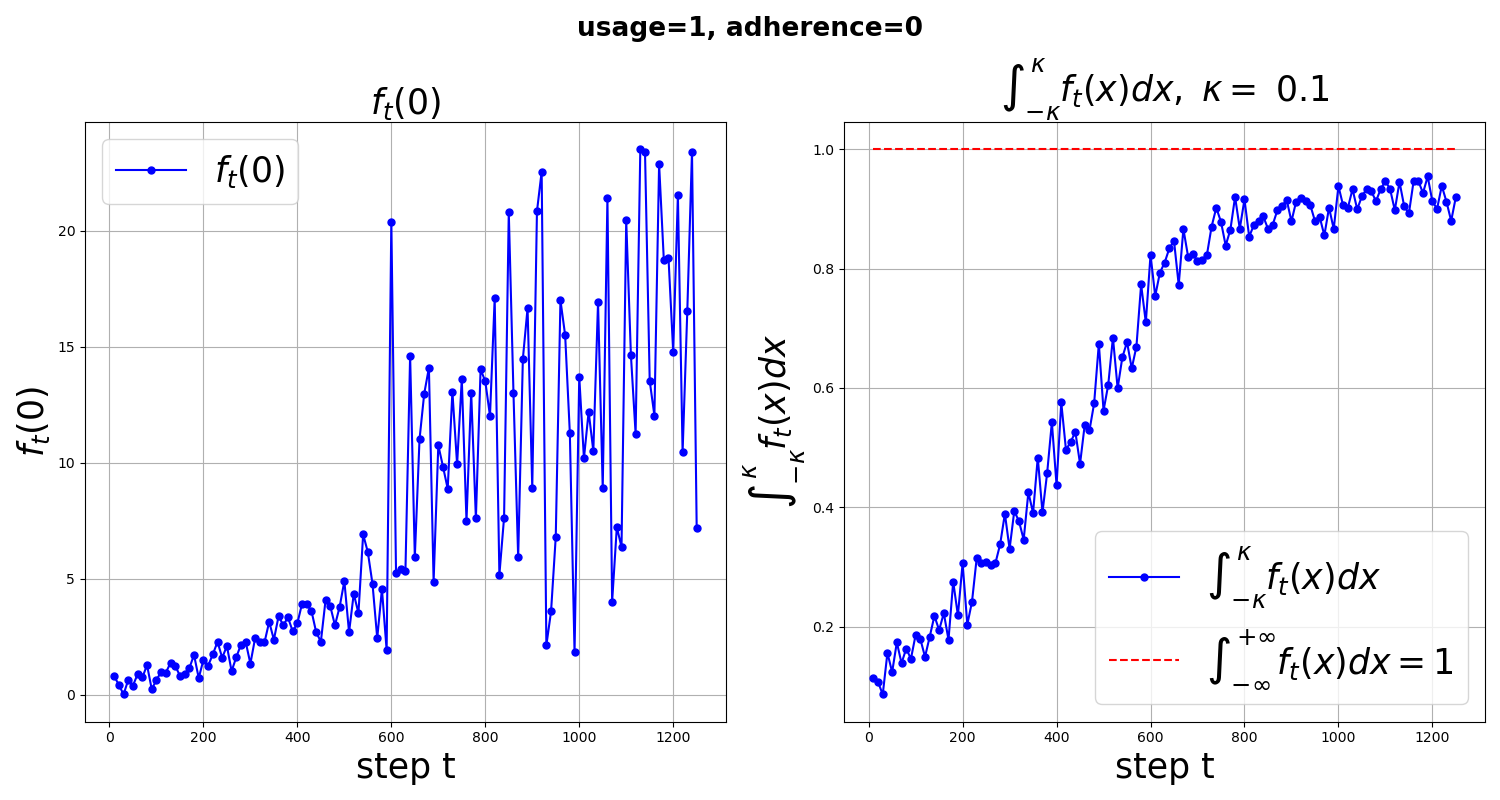
\includegraphics[width=0.4\linewidth]{pictures/ft0_loop_1_0.png}
            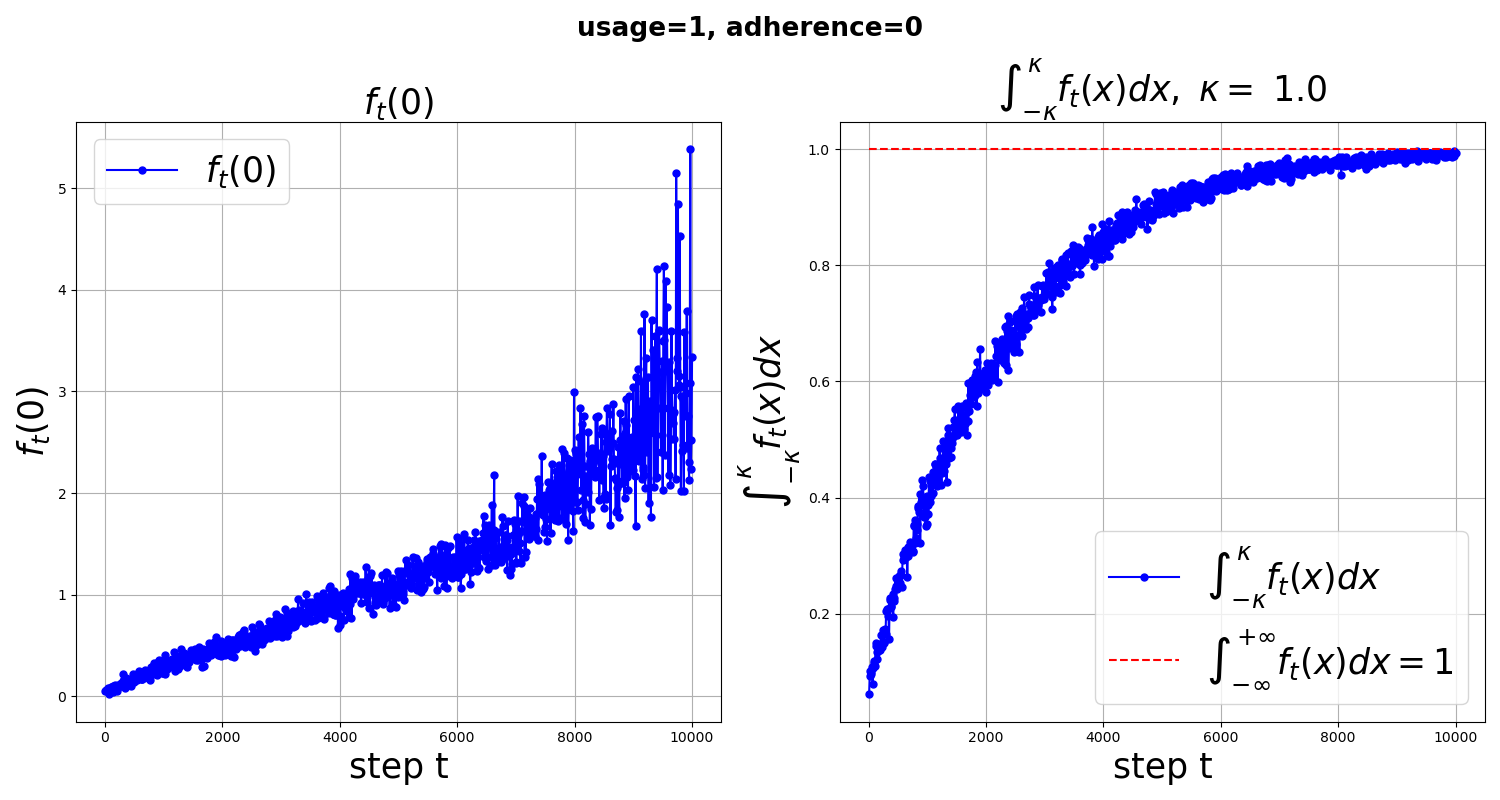
\includegraphics[width=0.4\linewidth]{pictures/ft0_sample_1_0.png}
                    
            \caption{Limit to delta function. Sliding window (left), sampling update (right).}
            
            \label{delta_loop}
        \end{figure}

        \begin{enumerate}
            \item Sliding window: $f_t(0)$ rises initially, then goes into a plateau.

            \item Sample update: $f_t(0)$ rises at all $t$.
        \end{enumerate}
        
    \end{frame}

    \begin{frame}{Autonomy check}
        \small
        In this experiment we test our system for autonomy, that is, we test the condition \eqref{cong_semigroup} in the Corollary 2. According to \eqref{cong_semigroup} $\psi(t)$ should be a power function, so we measured $\ln(f_t(0))$ and r2-score of it.

        \begin{figure}[h!]
            \centering
            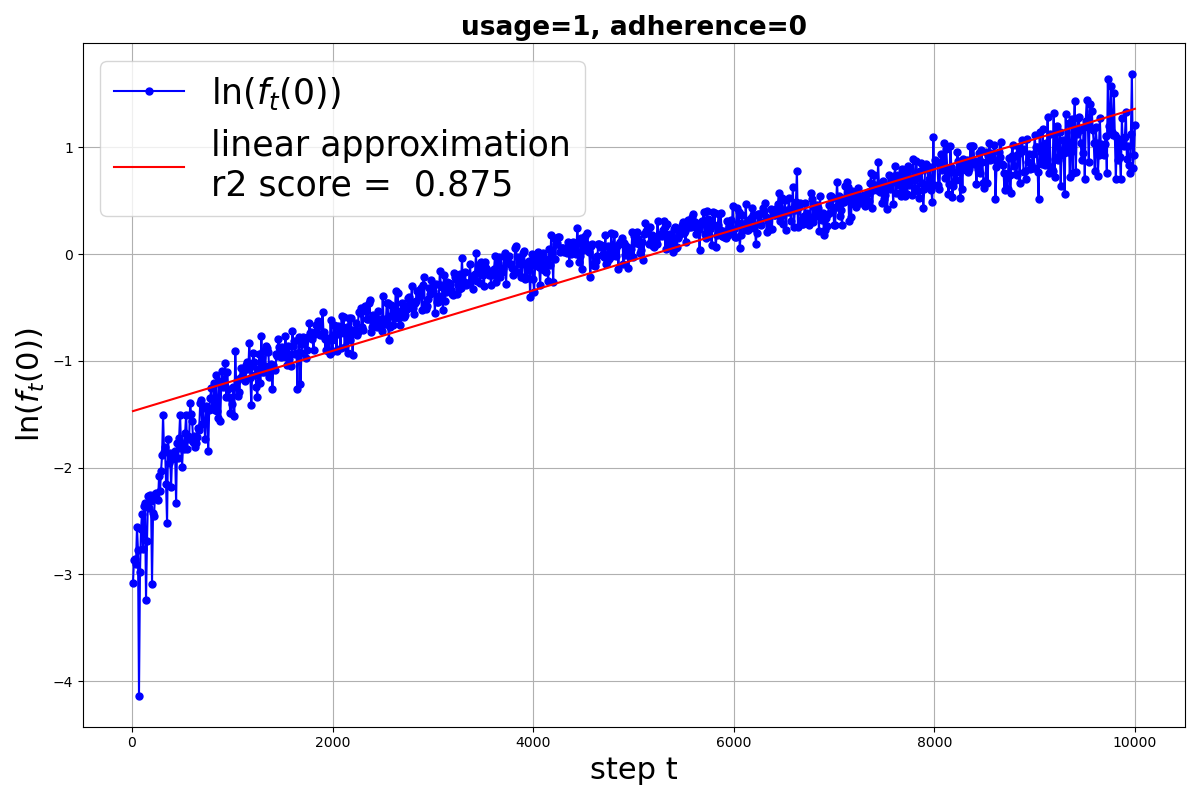
\includegraphics[width=0.32\linewidth]{pictures/semigroup_sample_1_0.png}
            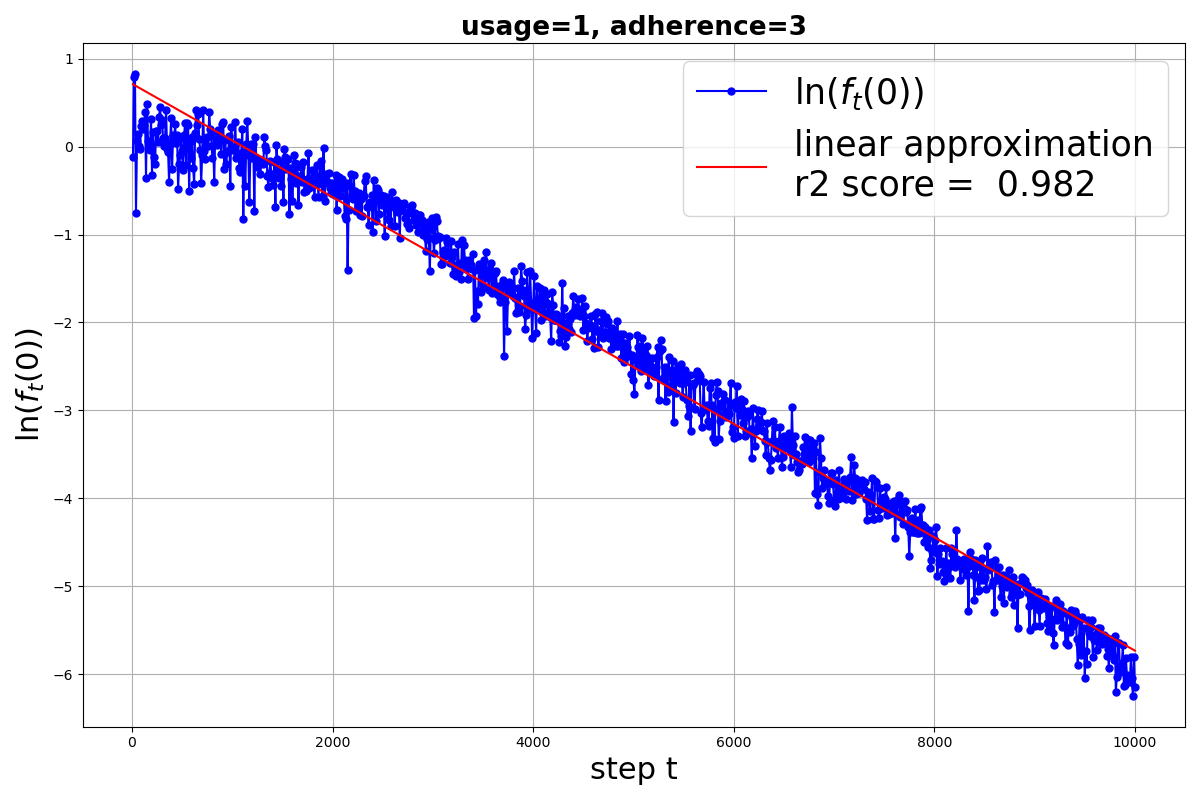
\includegraphics[width=0.32\linewidth]{pictures/semigroup_sample_1_3.png}
            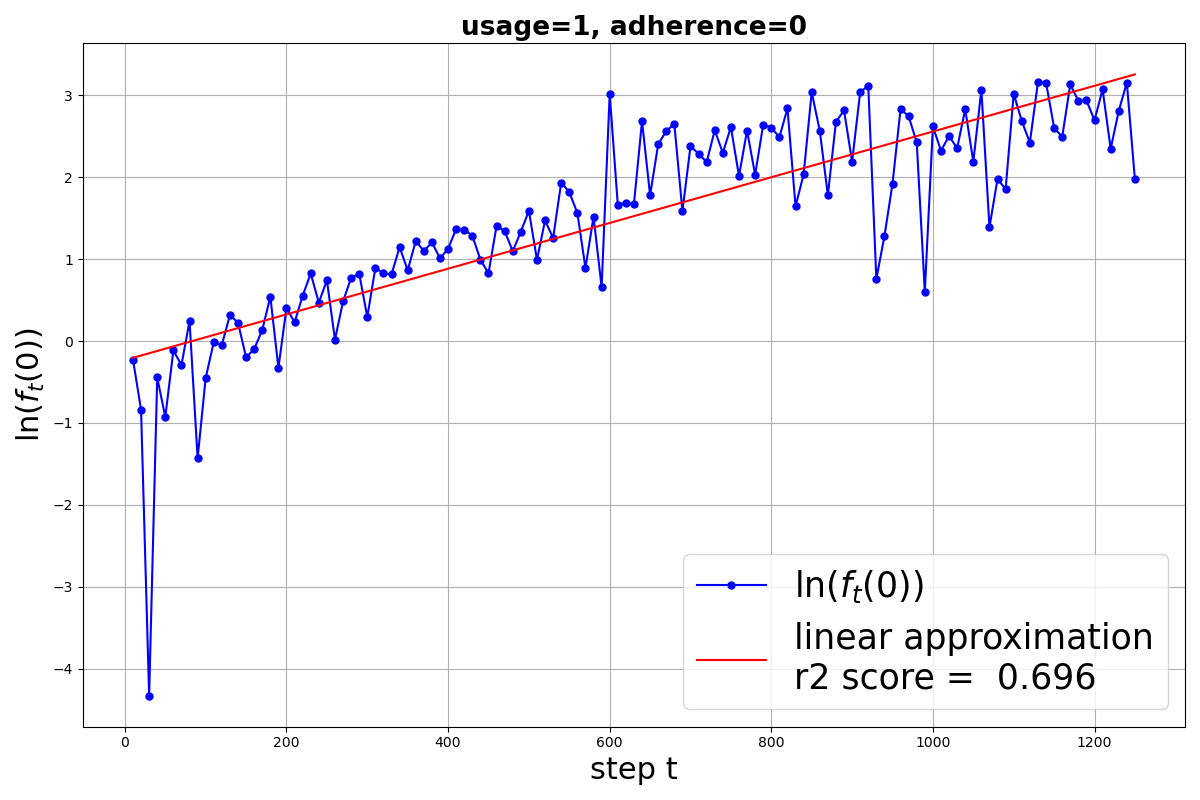
\includegraphics[width=0.32\linewidth]{pictures/semigroup_loop_1_0.png}
            
            \caption{Autonomy check. Sampling update (left and middle) and sliding window (right).}
            \label{fig_exp_4}
        \end{figure}

        \begin{enumerate}
            \item Sample update: r2-score is $0.875$ and $0.982$, so we can consider this system as autonomic

            \item Sliding window: r2-score is $0.696$ and points after $t > 600$ don't look like a line, so we can't consider this system as autonomic
        \end{enumerate}
    \end{frame}

    \begin{frame}{Decreasing moments}
        \small
        In this experiment we test the results from Corollary 3. In sampling update experiment we checked the first term of this Lemma, and in sliding window experiment we checked the second term.

        \begin{figure}[h!]
            \centering
            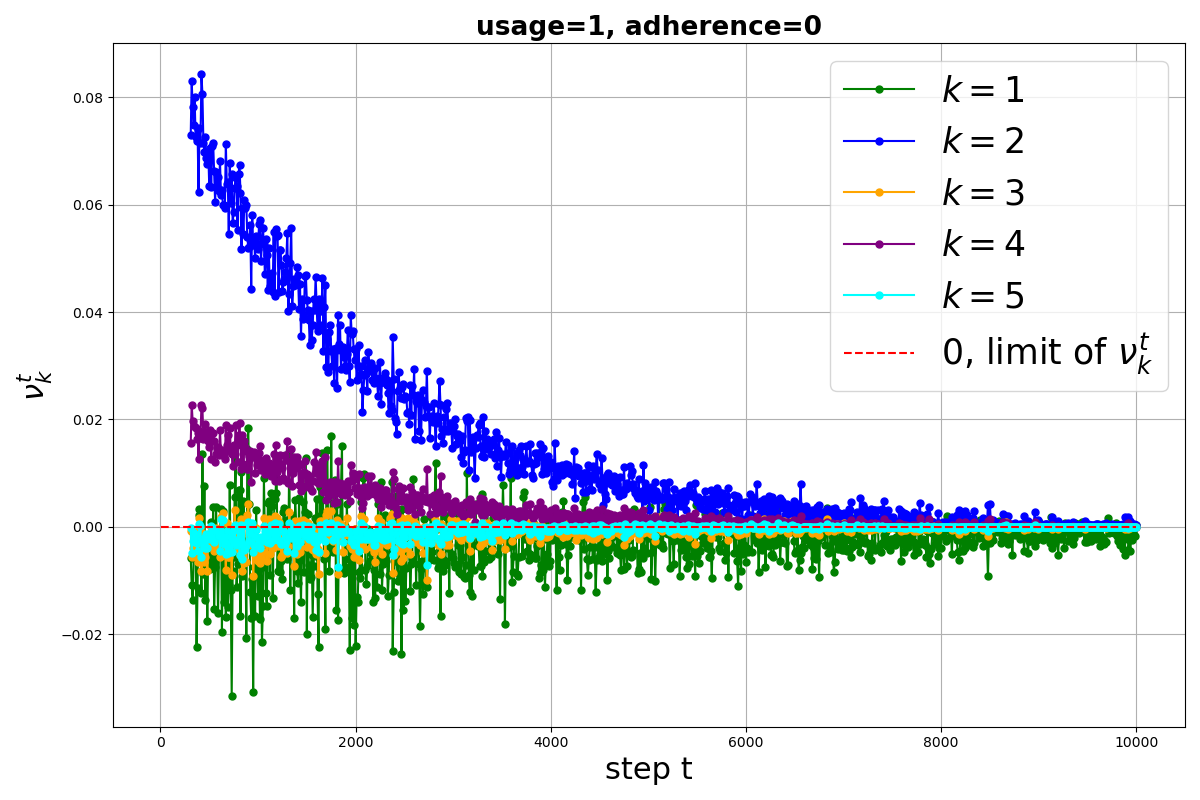
\includegraphics[width=0.4\linewidth]{pictures/moments_sample_1_0.png}
            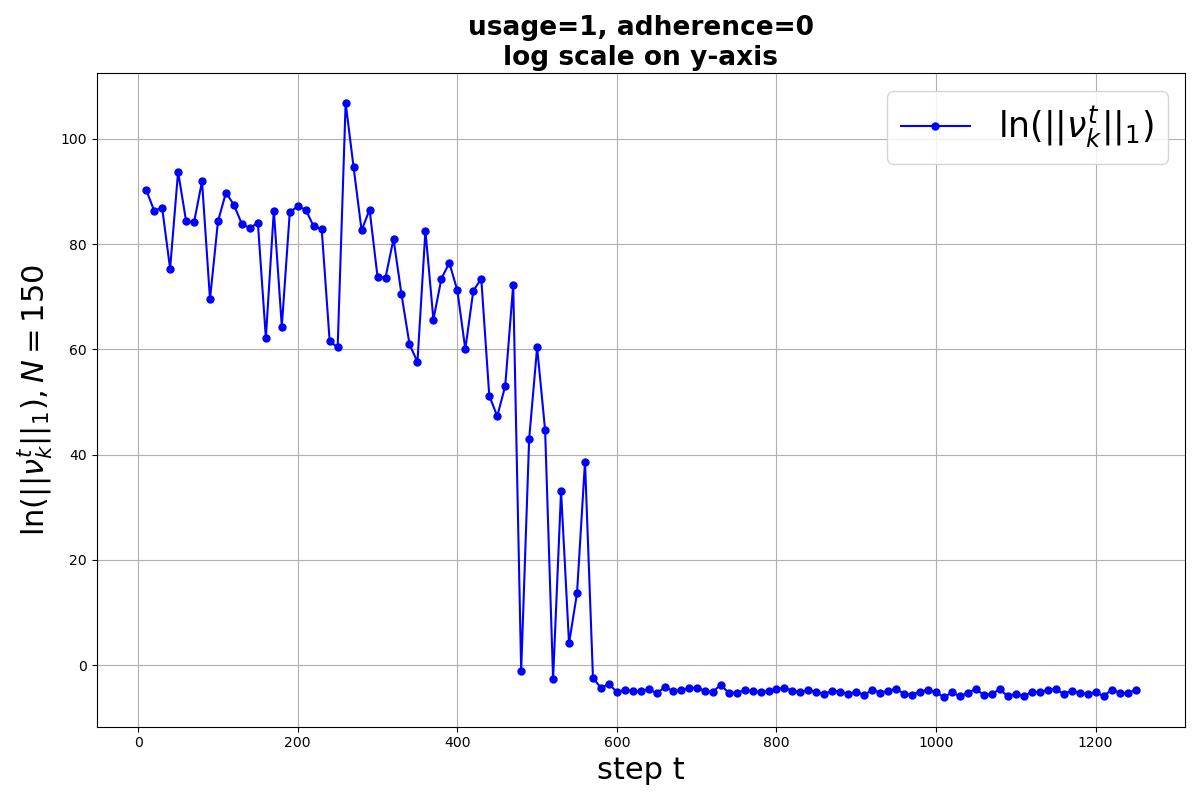
\includegraphics[width=0.4\linewidth]{pictures/moments_loop_1_0.png}
            
            \caption{Decreasing moments. Sampling update (left) and sliding window (right)}
            \label{fig_exp_5}
        \end{figure}

        As you can see, the moments tend to $0$, since the condition that $D^t(f_0)(x) \underset{t \to \infty}{\longrightarrow} \delta(x)$ is fulfilled
    \end{frame}

\section{Conclusion}

    \begin{frame}{Conclusion}
        \begin{enumerate}
            \item In this paper, we applied the apparatus of discrete dynamical systems, mathematical analysis and probability theory to build a theoretical framework in the problem of repeated supervised learning

            \item All results obtained are strongly proven and tested in a computational experiment

            \item We made a simulated environment in the Python language to build a simulation model of repeated supervised learning
        \end{enumerate}
    \end{frame}

\section{References}
    \begin{frame}{References}
        \tiny
        \bibliographystyle{plain}
        \bibliography{refs}  
    \end{frame} 

\end{document}
